%%	SECCION documentclass																									 %%	
%%---------------------------------------------------------------------------%%
\documentclass{report}

%%---------------------------------------------------------------------------%%
%%	SECCION usepackage																											 %%	
%%---------------------------------------------------------------------------%%
\usepackage{amsmath, amsthm}
\usepackage[spanish,activeacute]{babel}
\usepackage{caratula}
\usepackage{a4wide}
\usepackage{hyperref}
\usepackage{fancyhdr}
% \usepackage{moreverb}
\usepackage{graphicx} % Para el logo magico!
\usepackage{capt-of}
\usepackage{afterpage}
\usepackage{float}
\usepackage{amssymb}
\usepackage{amsmath}
\usepackage[latin1]{inputenc}
\usepackage{subfigure}
\usepackage{algorithm}
\usepackage{algorithmic}
\usepackage[dvipsnames,usenames]{color}
\usepackage{amsfonts}
%%---------------------------------------------------------------------------%%
%%	SECCION opciones																												 %%	
%%---------------------------------------------------------------------------%%
\parskip    = 11 pt
\headheight	= 13.1pt
\pagestyle	{fancy}
\definecolor{orange}{rgb}{1,0.5,0}

\addtolength{\headwidth}{1.0in}

\addtolength{\oddsidemargin}{-0.5in}
\addtolength{\textwidth}{1.0in}
\addtolength{\topmargin}{-0.8in}
\addtolength{\textheight}{0.7in}

%%---------------------------------------------------------------------------%%
%%	SECCION document	 %%	
%%---------------------------------------------------------------------------%%
\begin{document}
\renewcommand{\chaptername}{Parte }
\renewcommand{\algorithmicrequire}{\textbf{Requiere:}}
\renewcommand{\algorithmicensure}{\textbf{Asegura:}}
\renewcommand{\algorithmicend}{\textbf{Fin}}
\renewcommand{\algorithmicif}{\textbf{Si}}
\renewcommand{\algorithmicthen}{\textbf{entonces}}
\renewcommand{\algorithmicelse}{\textbf{Si no}}
\renewcommand{\algorithmicelsif }{\textbf{Si no y}}
\renewcommand{\algorithmicendif}{\textbf{Fin si}}
\renewcommand{\algorithmicfor}{\textbf{Ciclo}}
\renewcommand{\algorithmicendfor}{\textbf{Fin ciclo}}
\renewcommand{\algorithmicwhile}{\textbf{Mientras}}
\renewcommand{\algorithmicendwhile}{\textbf{Fin mientras}}

%%---- Caratula -------------------------------------------------------------%%
\materia{Algoritmos III}
\titulo{Trabajo Pr'actico n� 3}
%\subtitulo{Esp\'ia por error (num\'erico) }

\integrante{Gonz'alez, Emiliano}{426/06}{xjesse\_jamesx@hotmail.com}
\integrante{Gonz'alez, Sergio}{481/06}{gonzalezsergio2003@yahoo.com.ar}
\integrante{Mart'inez, Federico}{17/06}{federicoemartinez@gmail.com}
\integrante{Sainz-Tr'apaga, Gonzalo}{454/06}{gonzalo@sainztrapaga.com.ar}
\grupo{Grupo 3}
% FIXME: completar esto
\resumen{
}

% TOC, usa estilos locos
\maketitle
\pagestyle{empty}
{
\fancypagestyle{plain}
    {
    \fancyhead{}
    \fancyfoot{}
    \renewcommand{\headrulewidth}{0.0pt}
    } % clear header and footer of plain page because of ToC
\tableofcontents
}


\newpage
% arreglos los estilos para el resto del documento, y
% reseteo los numeros de pagina para que queden bien
\pagenumbering{arabic}
\fancypagestyle{plain} {
    \fancyhead[LO]{Gonz�lez, Gonz�lez, Mart�nez, Sainz Tr�paga}
    \fancyhead[C]{}
    \fancyhead[RO]{P\'agina \thepage\ de \pageref{LastPage}}
    \fancyfoot{}
    \renewcommand{\headrulewidth}{0.4pt}
}
\pagestyle{plain}
\chapter{Consideraciones preliminares}
\section{Descripci�n del problema}
\subsection{Aplicaciones practicas}

\section{Conteo de cruces}
\label{conteoCruces}
\subsection{Distintos algoritmos}
Dentro del problema que tenemos que resolver, un tema a tener en cuenta es el del conteo de cruces, ya que tanto la soluci�n exacta,
como las heuristicas necesitan saber muchas veces (por ejemplo para decidir donde se inserta un nodo, o si una permutaci�n ya no puede ser soluci�n) cuantos cruces hay en el dibujo. Por esta raz�n consideramos que un aspecto importante a optimizar para lograr mejorar el desempe�o de nuestros algoritmos es precisamente el conteo de cruces.

Lo primero que se puede observar es que los cruces en el dibujo depende solamente de la posici�n relativa de los nodos en las particiones. Se produce un cruce si hay dos nodos en una partici�n $v_i$, $v_j$ que estan relacionados con un $w_k$ y $w_p$ respectivamente tal que $v_i$ esta ``$arriba$'' de $v_j$ y $w_k$ esta ``$abajo$'' de $w_p$, como se ve en \ref{unCruce}.

\begin{figure}[H]
    \centering
     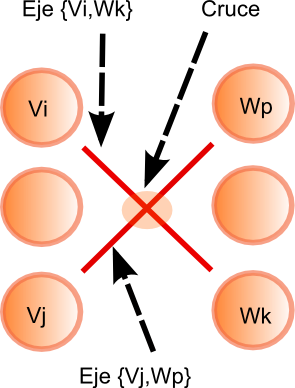
\includegraphics[scale=0.3]{./figuras/cruces/cruce.png}
     \caption{esquema de un cruce}
     \label{unCruce}
\end{figure}

Podemos entonces caracterizar en que casos se producen cruces:\\
\textit{Dado un orden de los nodos $p_1=<v_1,v_2,...,v_n>$ en una partici�n y un orden $p_2=<w_1,w_2,...,w_q>$ en la otra partici�n , se produce un cruce si existen ejes $(v_i,w_j)$, $(v_k,w_p)$ tal que $i<k \wedge p<j$.}

De esta manera un primer algoritmo para contar los cruces, consiste en tomar cada par de ejes y comparar las posiciones relativas de sus nodos.
Hacer esto tiene un costo $\theta(m^2)$, siendo $m$ la cantidad de ejes, ya que la cantidad de posibles pares de ejes es $\binom{m}{2} = \frac{m*(m-1)}{2}$. Este costo puede ser excesivo, principalmente en grafos densos, donde m puede ser del orden de $n_1*n_2$, siendo $n_i$ la cantidad de nodos en las particion i.

Buscamos entonces alg�n algoritmo que nos de un orden mejor que $O(m^2)$\footnote{cuando hablamos de complejidad en el �mbito del conteo de cruces, nos referimos a complejidad en el modelo uniforme}. 

Si se ordenan los ejes del grafo primero por su componente en la particion $p_1$ y luego por su componente $p_2$, es decir si $e_i=(i_1,i_2)$ y $e_j=(j_1,j_2)$ son ejes del grafo, consideramos que $e_i < e_j \Leftrightarrow i_1 < j_1 \vee (i_1 == j_1 \wedge i_2 < j_2)$ y consideramos luego el orden en el que quedan las segundas componentes, podemos ver que cada inversi'on es un cruce. Una inversi�n en el orden $\pi=<a_1,a_2,....a_n>$ es un par $(a_i,a_j)$ tal que $a_i > a_j$ $\wedge$ $i<j$. 

Decimos que una inversi�n representa a un cruce porque como primero se ordena por la primer componente (en verdad es la componente de la primer partici�n, pero para simplificar la notaci�n nos referiremos a dicha componente como la primer componente) y luego por la segunda, si hay una inversion es porque para los ejes $(v_k,a_i)$ y $(v_p,a_j)$ val�a que $v_k < v_p \wedge a_i > a_j$, y esa es la condici�n para que se produzca un cruce.

%TODO: ver si no hay q explicar mejor como se puede calcular eso
Entonces si ordenamos los ejes de esa manera y despu�s contamos las inversiones, podemos obtener el numero de cruces. Para ordenar a los ejes se puede utilizar radix sort, suponiendo que los ejes tienen como componentes las posiciones relativas de los nodos (o que estas se pueden obtener), lo cual se puede calcular en caso de que esa informaci�n no este disponible con un costo de $n_1 + n_2 + m $, con $n_i$ la cantidad de nodos de la partici'on i, obteniendo los indices de los nodos en cada particion y luego usando esta informaci�n ``traducir'' los ejes; y luego consideramos el arreglo que tiene a las segundas componentes de los ejes como elementos, aplicar insertion sort y por cada cambio de posici�n que se hace para un elemento, contar una inversi�n y por lo tanto un cruce. Esto �ltimo tendr�a un costo $O(m+c)$, con c la cantidad de cruces. En el peor caso, todos los ejes se cruzan por lo que tendr�amos un costo $O(m^2)$ nuevamente.

Veamos un ejemplo de como funciona este algoritmo:
Consideremos el siguiente grafo bipartito:
\begin{figure}[H]
    \centering
     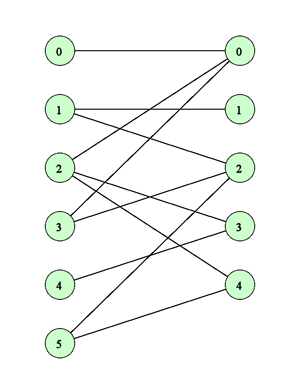
\includegraphics[scale=0.8]{./figuras/cruces/ejemplo1.png}
     \caption{Grafo de ejemplo para la aplicacion de los algoritmos de conteo de cruces}
     \label{ejemplo1}
\end{figure} 

Ahora ordenamos los ejes de acuerdo a su primer componente y luego a su segunda, obtenemos lo siguiente:

$$\left\langle (0,0),(1,1),(1,2),(2,0),(2,3),(2,4),(3,0),(3,2),(4,3),(5,2),(5,4)\right\rangle$$

Entonces el arreglo formado por las segundas componentes es el siguiente:

$$\left\langle0,1,2,\textcolor{Red}{0},3,4,0,2,3,2,4\right\rangle$$

Entonces, aplicamos selection sort. El 0 (de color rojo),recorre dos posiciones antes de insertarse en su posici�n correcta.

$$\left\langle0,0,1,2,3,4,\textcolor{Red}{0},2,3,2,4\right\rangle$$

Luego el tercer 0 se swapea cuatro veces:
 
$$\left\langle0,0,0,1,2,3,4,\textcolor{Red}{2},3,2,4\right\rangle$$

El segundo 2 cambia dos veces de posici�n:

$$\left\langle0,0,0,1,2,2,3,4,\textcolor{Red}{3},2,4\right\rangle$$

Ahora el segundo 3 cambia una vez de posici�n:

$$\left\langle0,0,0,1,2,2,3,3,4,\textcolor{Red}{2},4\right\rangle$$

Finalmente el �ltimo 2 es swapeado tres posiciones.

Entonces la cantidad de cruces del grafo es: $2+4+2+1+3 = 12$

Si bien en el caso general este algoritmo tiene un mejor orden, en peor caso sigue siendo $O(m^2)$.

Veamos un tercer acercamiento al problema: Sea $\sharp v_2$ la cantidad de nodos de la particion 2. Consideremos un arbol binario con $2^k$ hojas donde k es tal que $2^{k-1} < \sharp v_2 <= 2^{k}$ de modo de que cada nodo este en una hoja (podria haber hojas que no tengan a ningun nodo), dispuestos de izquierda a derecha seg�n su orden en la partici�n. Este �rbol tiene $2^{k+1}-1$ nodos. Ademas $k=\left\lceil log_{2}(\sharp v2)\right\rceil$

Lo que vamos a hacer es ordenar a los ejes como lo hicimos para el algoritmo anterior. Luego lo que haremos es agregar a los ejes segun dicho orden. Agregar el eje consiste en incrementar en uno el contador, en principio inicializado en 0, de la hoja correspondiente al nodo de la segunda componente del eje. Ademas se incrementa tambi�n en uno el contador del padre de dicha hoja y este incremento se va propagando hacia arriba hasta la ra�z.

Cada vez que insertamos un eje, en cada nivel, si estamos parados en un nodo izquierdo aumentamos el n�mero de cruces seg'un el valor del hermano del nodo.

El procedimiento puede resultar confuso en un principio por lo cual mostraremos un ejemplo de su aplicaci�n.
Apliquemos el algoritmo para el grafo de \ref{ejemplo1}:

Como tenemos $\sharp v_2 = 5$, el arbol va a tener 8 hojas y un total de 15 nodos.
 
\begin{figure}[H]
    \centering
     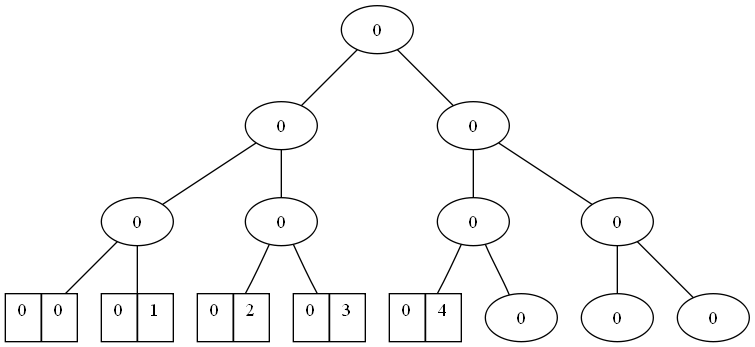
\includegraphics[scale=0.4]{./figuras/cruces/arbol.png}
     \caption{�rbol para contar cruces en el grafo de ejemplo}
     \label{arbol}
\end{figure} 

Los nodos cuadrados (del 'arbol) son las hojas que representan al nodo (del grafo bipartito) cuyo numero es el de la derecha de la hoja. Cada nodo tiene un contador , en principio inicializado en 0. El contador de cruces tambi�n esta inicializado en 0.

Recordemos que luego de ordenar los ejes el vector era:
$$\left\langle(0,0),(1,1),(1,2),(2,0),(2,3),(2,4),(3,0),(3,2),(4,3),(5,2),(5,4)\right\rangle$$

Lo primero que hacemos entonces es insertar el eje (0,0), de modo que se incrementa el contador de la hoja 0 y este incremento se propaga hacia arriba. Como 0 esta en un nodo izquierdo, lo que se hace es sumar a la cantidad de cruces el valor del contador del hermano de 0 (la hoja 1). Esto porque, porque el valor de dicho contador indica la cantidad de ejes insertados que terminaban en 1, pero ademas dado el orden que se usa para agregar a los nodos, sabemos que la primer coordenada de estos ejes que terminaban en 1 era menor que la del ejes que estoy insertando ahora, por lo tanto hay un cruce. En otras palabras, agregue un eje (a,1) antes que uno (b,0) y por como estban ordenados los nodos, sabemos que $a<b$ y como $1>0$, hay una inversi�n.

Al subir de nivel, como tambi�n estamos en un nodo izquierdo, agregamos a la cantidad de cruces el valor del contador del hermano correspondiente. En este caso, dicho contador guarda la cantidad de ejes agregados que terminan en 2 0 3. Y asi sucesivamente hasta la ra�z. 

Luego de esta inserci�n obtenemos el siguiente �rbol:
\begin{figure}[H]
    \centering
     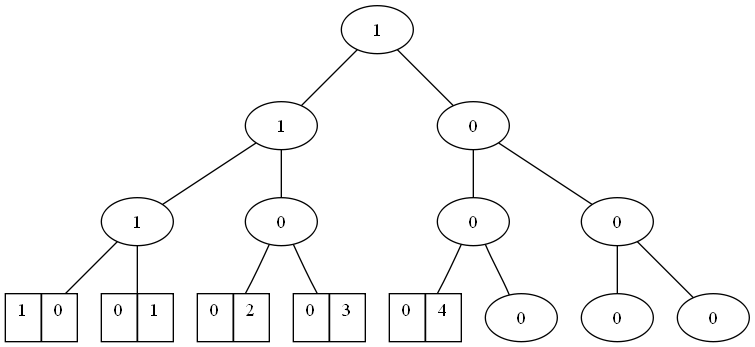
\includegraphics[scale=0.4]{./figuras/cruces/arbol2.png}
     \caption{�rbol con el eje (0,0) insertado}
     \label{arbol2}
\end{figure} 

De manera analoga, se insertan los ejes (1,1) y (1,2), sin que se generen cruces, en este caso el arbol queda de la siguiente manera:

\begin{figure}[H]
    \centering
     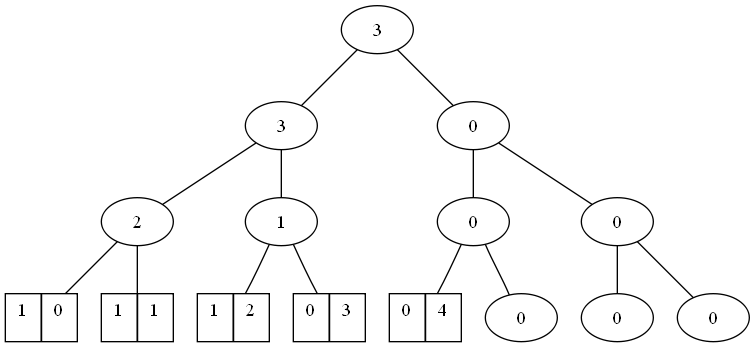
\includegraphics[scale=0.4]{./figuras/cruces/arbol3.png}
     \caption{�rbol con los ejes (0,0),(1,1) y (1,2) insertados}
     \label{arbol3}
\end{figure} 

Luego corresponde insertar el eje (2,0). Incrementamos en uno el contador de la hoja 0. Como es un nodo izquierdo, sumamos a cantidad de cruces el valor de la hoja 1, que es 1. Este incremento corresponde al cruce del eje (2,0) con el eje (1,1). Subimos un nivel e incrementamos en 1 el contador del padre de la hoja 0. Nuevamente sumamos al contador de cruces, el valor del contador del hermano del nodo donde estamos parados, ya que otra vez estamos en un nodo izquierdo. Este nuevo incremento corresponde al cruce entre el eje (2,0) y el eje (1,2). Seguimos subiendo hasta llegar a la ra�z, incrementando el valor de los contadores y en el caso de pasar por un nodo izquierdo, sumando el valor de los contadores de los nodos derechos. En particular en este caso, volvemos a caer en un nodo izquierdo, pero el contador de su hermano es 0. Esto se debe a que todavia no insertamos ning�n eje que terminara en 4.

\begin{figure}[H]
    \centering
     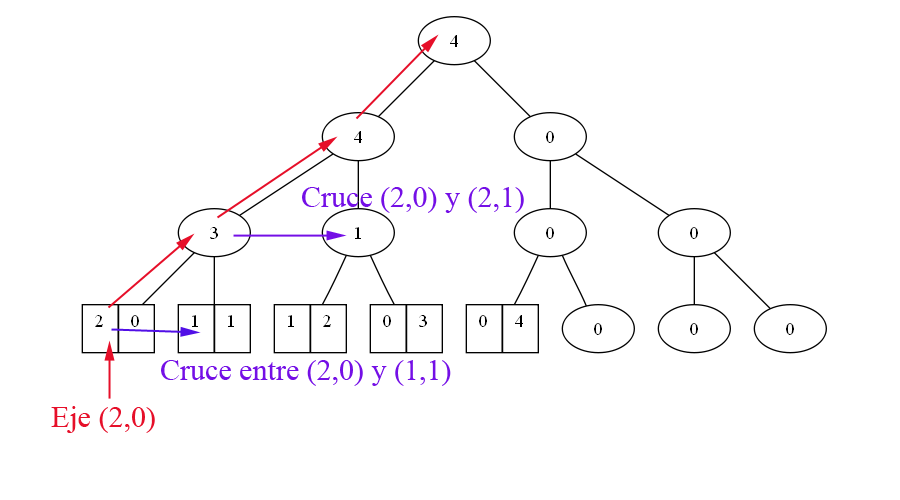
\includegraphics[scale=0.4]{./figuras/cruces/arbol4.png}
     \caption{�rbol con los ejes (0,0),(1,1),(1,2) y (2,0) insertados}
     \label{arbol4}
\end{figure} 


El procedimiento se repite hasta colocar todos los ejes.

Como veremos mas adelante, este procedimiento tiene como orden $O(max(m,\sharp v_1, \sharp v_2)+m*log(min_{i=1,2}(\sharp(v_i))))$

Repasando tenemos 3 algoritmos para calcular los cruces:
\begin{itemize}
\item El primero, consiste en revisar todo par de ejes. Tiene un costo $O(m^2)$
\item El segundo ordena los ejes y luego realiza insertion sort para contar inversiones. Tiene un costo de $O(max(m,\sharp v_1, \sharp v_2)+c)$
\item El tercero utiliza el arbol binario para contar inversiones. Tiene un orden $O(max(m,\sharp v_1, \sharp v_2)+m*log(min_{i=1,2}(\sharp(v_i))))$
\end{itemize}

Todas estos algoritmos requieren conocer el ``orden'' de los nodos en cada particion, lo cual podria hacerse, en $O(\sharp(v_1) + \sharp(v_2))$ costo que se suma a los algoritmos en caso de que no se tenga dicha informaci�n.

Si $m > log(min_{i=1,2}(\sharp(v_i)))$ conviene utilizar el tercer algoritmo, pues tiene una complejidad menor que la de los otros dos.

Si en cambio $m < log(min_{i=1,2}(\sharp(v_i)))$ (un grafo con muy pocos ejes) resulta conveniente utilizar el segundo algoritmo ya que provee un mejor orden.

Sin embargo, podemos evitar los casos donde se tengan pocos ejes. Para hacerlo, preprocesamos el grafo, de modo de sacar los nodos aislados, ya que estos se pueden insertar en cualquier lado sin que agreguen cruces.En el caso de un nodo del grafo original, si bien no puede insertarse en cualquier lado en el sentido estricto, vale que no suma cruces igualmente, por lo cual se lo puede sacar para aplicar cualquier algoritmo y luego insertarlo en la soluci�n en una posici�n valida.

De esta manera, el algoritmo 3 se muestra como la mejor opci�n, ya que si $m>\sharp v_i$, resulta que $O(max(m,\sharp v_1, \sharp v_2)+m*log(min_{i=1,2}(\sharp(v_i)))) \subseteq O(m*log(min_{i=1,2}(\sharp(v_i))))$.

\subsubsection{Pseudocodigo}
\begin{algorithm}[H]
\caption{Cuenta los cruces en un dibujo usando un arbol acumulador}
\begin{algorithmic}[1]
\PARAMS{particiones del dibujo (suponemos para simplificar que p2 tiene menos nodos (o igual cantidad) que p1)}
\PARAMS{los ejes del dibujo,las posiciones (indice) de los nodos}
\STATE ejsPorPos $\leftarrow$ $[]$
\FOR{cada eje(x,y) del dibujo}
\STATE agregar a ejesPorPos la tupla (posicion de x, posicion de y)
\ENDFOR
\STATE lista $\leftarrow$ RadixSort de los ejes de ejesPorPos de modo que (x,y) $<$ (z,w) si $x < z \vee x = z \wedge y < w$
\STATE primerIndice $\leftarrow$ $2^{ \left\lceil log_{2}(largo de p2) \right\rceil }$
\STATE arbol $\leftarrow \underbrace{[0,...,0]}_{2*primerIndice - 1}$
\STATE \COMMENT{arbol es el arbol acumulador}
\STATE decrementar primerIndice
\STATE cruces $\leftarrow$ 0
\FOR{cada eje de la lista}
\STATE indice $\leftarrow$ segunda componente del eje + primerIndice
\STATE arbol[indice] $\leftarrow$ arbol[indice] + 1 \COMMENT{un eje mas en esta hoja}
\WHILE{ indice $>$ 0}
\IF{indice es impar}
\STATE \COMMENT{estoy en un nodo izquierdo}
\STATE cruces $\leftarrow$ cruces + arbol[indice]
\ENDIF
\STATE indice $\leftarrow$ $(indice -1)/2$ \COMMENT{subo un nivel}
\STATE arbol[indice]~$\leftarrow$ arbol[indice] + 1
\ENDWHILE
\ENDFOR
\RETURN cruces
\end{algorithmic}
\end{algorithm} 

\subsection{Calculo de complejidad}
Sea $v_i$ la cantidad de nodos de la particion i, y m la cantidad de ejes del grafo.

Si bien comentamos que la funci�n podr�a en caso de que no este disponible calcular los indices de los elementos, esta funcionalidad no fue utilizada, de modo que el algoritmo recibe los indices ya armados. De este modo, el costo de armar y manter a los indices sera tenido en cuenta en los respectivos algoritmos que utilicen a esta funci�n.

Primero lo que hacemos es traducir los ejes, segun los indices. Para hacer esto, lo que se hace es recorrer todos los ejes (se recorren las listas de adyacencia de los nodos de una de las particiones) y se van guardando en una lista, los ejes con sus compoentes traducidas (ciclo de la l�nea 2).

Luego ordenamos los ejes, como lo hacemos con radix sort, el costo es $max(m, v_1, v_2)$, puesto que tengo que ordenar m ejes, y para hacerlo voy a necesitar de $\sharp v_1$ $buckets$ primero y $\sharp v_2$ $buckets$ luego.

Una vez ordenado y armado el 'arbol, que se puede hacer en O($v_2$) como se vera mas adelante, vamos a mirar todos los ejes. Para cada eje recorremos el arbol desde una hoja hasta la raiz. Como el arbol tiene $2^k$ hojas, tiene $log_{2}(2^k)$ de altura, pero $log_{2}(2^k)=k=\left\lceil log_{2}(\sharp v2)\right\rceil$.

El arbol se puede implementar sobre un arreglo, de modo que la posici�n 0 sea la ra�z, la 1 y 2 sus hijos izquierdo y derecho respectivamente, y asi sucesivamente (de manera analoga a como se hace para implementar un heap). De esta manera, los nodos izquierdos del �rbol quedan en las posiciones impares, y aumentar cada contador, asi como tambi�n moverse dentro del �rbol de un nodo a su padre se puede hacer en O(1). Por lo tanto, el costo de insertar todos los ejes es $O(max(m,\sharp v_1, \sharp v_2)+m*log(\sharp v_2) )$.

\begin{figure}[H]
    \centering
    \subfigure[�rbol acumulador]{
     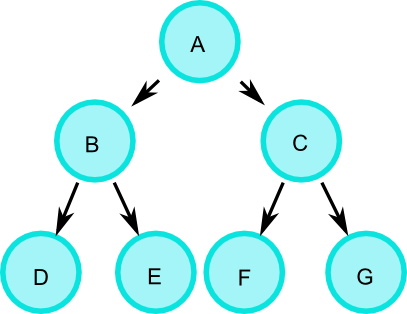
\includegraphics[scale=0.2]{./figuras/cruces/arbolito.png}}
     \subfigure[Representaci�n en arreglo]{
     
\includegraphics[scale=0.2]{./figuras/cruces/arreglito.png}}

\end{figure} 

Ahora bien, en vez de ordenar primero por la primer componente y luego con respecto a la segunda, podr'iamos hacer el mismo procedimiento pero ordenando primero por la segunda, luego por la primera y armando el arbol para $v_1$. Entonces, en particular el procedimiento se podria realizar utilizando el  $v_i$ de menor cardinal. Con lo cual el costo de las inserciones es de $O(max(m,\sharp v_1, \sharp v_2)+m*log(min_{i=1,2}(\sharp v_i) ))$

Como dijimos, este algoritmo podria no ser eficiente si la cantidad de ejes es muy peque�a, ya que para hacer radix sort se van a recorrer todos los nodos de ambas particiones, lo cual podria ser un costo mas grande que mirar todos los ejes. Sin embargo, tambi�n comentamo que vamos a filtrar a los nodos de grado 0 antes de trabajar con el dibujo, por lo cual creemos que este algoritmo es eficiente. Filtrar a los nodos de grado 0 tiene sentido, ya que por ejemplo en nuestro algoritmo exacto, un peque�o incremento en la cantidad de nodos, siginifica un gran aumento en la cantidad de permutaciones, de esta manera si lo separamos el algoritmo no perderia tiempo en mover a este nodo que no genera cambio alguno.

\subsection{Reutilizaci�n de los c�lculos}
\label{reUso}
Si bien hay situaciones donde el orden relativo de los nodos en las particiones se podr�a modificar sustancialmente, por lo cual ser�a necesario recalcular los cruces nuevamente , lo cual, como vimos en la secci�n anterior, tiene un costo bastante alto; hay otros casos donde se hace una modificaci�n mas peque�a al orden de los mismos y es posible no recalcular todos los cruces.

En particular si tenemos un orden de los nodos $\pi=\left\langle v_1,v_2,...v_i,v_{i+1},...,v_n \right\rangle$ y realizamos un ``swap'' entre dos posiciones consecutivas $i$, $i + 1$, podemos observar que si $\pi_1=C(\left\langle v_1,v_2,...,v_{i+1},v_{i},...v_n \right\rangle$ y definimos C($\pi$,$\rho$) como la cantidad de cruces entre los ejes del grafo, dado que los nodos de la primer partici�n estan ordenados seg'un $\pi$ y los de la segunda segunda seg�n $\rho$, vale que:

 $$C(\pi_1,\rho) = C(\pi,\rho) - CrucesEntre(v_i,v_{i+1},\rho) + CrucesEntre(v_{i+1},v_i,\rho)$$

Donde CrucesEntre(a,b,$\rho$) es la cantidad de cruces entre ejes de $a$ y ejes de $b$ si $a$ esta en una posicion relativa menor que la de $b$ y dado que los nodos de la otra partici�n estan en el orden $\rho$. Esto se debe a que como dijimos anteriormente, los cruces dependen solo del orden relativo. Entonces si intercambiamos dos posiciones consecutivas, el orden relativo de los demas nodos se mantiene, es decir, los que estaban ``abajo'' de ellos siguen estando all�, y los que estaban ``arriba'' tambi�n, de modo que solo cambian los cruces que hay entre los dos nodos movidos.

\begin{figure}[H]
    \centering
    \subfigure[]{
     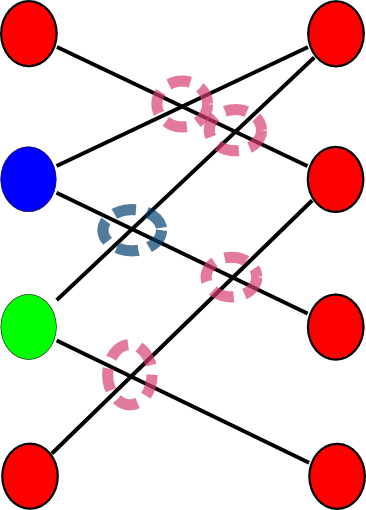
\includegraphics[scale=0.2]{./figuras/cruces/crucesPreSwap.png}}
     \subfigure[]{
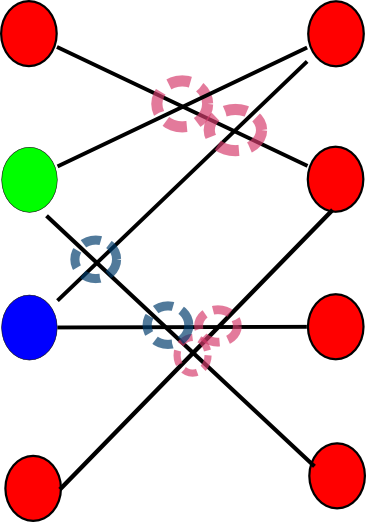
\includegraphics[scale=0.2]{./figuras/cruces/crucesPostSwap.png} }
     \label{fig:swap}
     \caption{Al intercambiar los nodos verde y azul, los cruces que involucran al resto de los nodos se mantienen}
\end{figure} 


Para calcular crucesEntre se puede utilizar el algoritmo antes descripto para el conteo de cruces en general, simulando una partici�n que solo contenga a los nodos $a$ y $b$, y solo teniendo en cuenta los ejes que salen de ellos dos. En este caso, como la partici�n mas chica tiene 2 nodos (o menos si una partici�n era solo un nodo), resulta que el algoritmo puede calcular los cruces en $O( v_j + m_{a} + m_{b})$ con $m_{a,b}$ la cantidad de ejes incidentes a $a$ y a $b$ y $v_j$ es la otra partici�n. Basicamente lo que hacemos solo mirar los ejes que salen de a y de b, armar un arbol de dos posiciones y aplicar el procedimiento anterior

%FIXME: Esto esta bien?
En el caso en que a y b tengan pocos ejes, de modo tal que $m_{a}*m_{b} < \sharp v_j$ , utilizamos la versi�n simple del algoritmo toma todos los pares de ejes de a y b. De este modo el orden para contar cruces es $min(max(v_j,m_a,m_b),m_a*m_b)$
 
\begin{figure}[H]
    \centering
    \setcounter{subfigure}{0}
    \subfigure[]{
     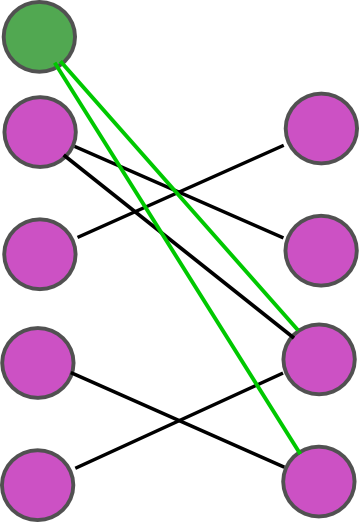
\includegraphics[scale=0.2]{./figuras/cruces/nuevoNodo.png}}
     \subfigure[]{
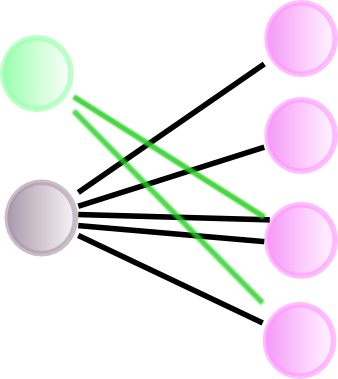
\includegraphics[scale=0.2]{./figuras/cruces/compactado.png} }
     \caption{Compactaci�n del grafo para averiguar cuantos cruces agrega un nuevo nodo}
     \label{fig:compactar}
\end{figure} 

Otro caso donde se puede evitar re calcular todos los cruces es cuando se agrega un nodo al dibujo, particularmente si se agrega al principio o al final de la partici�n. En este caso, los cruces existentes entre otros nodos se mantienen, solo se podr�an agregar nuevos cruces con los ejes del nodo recien agregado. Entonces podemos colapsar los nodos de la partici�n donde se esta agregando el nuevo nodo, dejando solo al nuevo nodo y a un nodo $w$ con todos los ejes del resto como ilustra la figura \ref{fig:compactar}, de modo de que el algoritmo sea $O(m + v_1+v_2 + m)$. Esto es asi porque el costo de la traducci�n y del radix sort hay que hacerlo igual, pero al igual que en el caso de los cruces entre dos nodos consecutivos, el arbol tiene solo 2 elementos: el nodo que se agrega y el nodo que compacta a todos los demas con sus ejes.

Estas situaciones si bien parecen casos muy especificos, pueden ser aprovechados por los distintos algoritmos que desarrollamos.

\section{Eliminaci�n de nodos nulos}
\label{sacoNulos}
Como dijimos, antes de aplicar las heuristicas, eliminamos los nodos de grado cero en lo que ser�a el grafo con todos los nodos ya puesto. Consideramos que esto evita que las heuristicas, asi como tambi�n el algoritmo exacto, realicen calculos innecesarios.

Para hacerlo, basicamente tomamos los nodos de la entrada, asi como sus ejes y construimos un dibujo. A partir de este dibujo, que ya tiene armadas las listas de adyacencia, podemos separar en una lista a los nodos de grado distinto a cero. 

\begin{figure}[H]
    \centering
    \setcounter{subfigure}{0}
    \subfigure[]{
     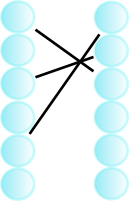
\includegraphics[scale=0.2]{./figuras/cruces/pocosEjes.png}}
     \subfigure[]{
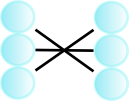
\includegraphics[scale=0.2]{./figuras/cruces/limpio.png} }
     \caption{Reducir la cantiidad de cruces en el primero es equivalente a hacerlo en el segundo}
     \label{fig:limpieza}
\end{figure} 

Si solamente los sacaramos, nos encontrar�amos frente al problema de que los nodos no tienen como identificadores n�meros consecutivos. Por esta raz�n, no solo filtramos a los nodos de grado nulo, sino que se realiza un nueva n�meraci�n de los nodos que quedan. La misma cumple que los nodos fijos tienen n�meraci�n consecutiva (la cual ademas indica la posici�n relativa, es decir si a $<$ b con a y b nodos de la misma partici�n, entonces el nodo fijo a esta antes que el nodo fijo b) y que los n�meros son asignados primero a los nodos fijos de la primer partici�n, luego a los nodos fijos de la segunda, en tercer lugar a los nodos no fijos de la primera y finalmente a los de la segunda.

Para realizar dicha traducci�n se utilizan diccionarios sobre arreglos a fin de poder realizarla rapidamente. Lo que se guarda es dado un identifador nuevo a que nodo viejo identifica. 

Los ejes tambi�n son traducidos, por lo cual se necesita momentaneamente poder ir de un identificador viejo a su numero nuevo, por lo cual se necesita otro indice provisioriamete.

Una vez que se realiz� la traducci�n, las heuristicas y el algoritmo exacto trabajan con el dibujo nuevo.

Cuando terminan se realiza el proceso inverso para volver de los nodos nuevos a los viejos, y ademas insertar a los viejos en posiciones validas (hay que respetar la posicon de los nodos fijos que ten�an grado cero y no fueron tenidos en cuenta)

Todo este proceso nos agrega un costo $O(V_1+V_2+m)$ donde $V_i$ es la cantidad de nodos de partici�n i sin filtrar y m la cantidad de ejes. En el peor caso, ning�n nodo ten�a grado cero, por lo que esta mejora representa un overhead, sin embargo como se ver� mas adelante el orden de los distintos algoritmos es lo suficientemente elevado como para hacer despreciable dicho overhead.

%TODO: comparar que pasa si no saco los nodos al pedo y si los saco

\newpage
\chapter{Conclusi�n}

\begin{thebibliography}{9}

\end{thebibliography}
\label{LastPage}
\end{document}
